\section{Fuerza eléctrica}

\subsection{Ley de Coulomb}

La electrostática estudia las cargas eléctricas en reposo. En definitiva, estudiará cargas que no se mueven, pero sienten fuerzas. La interacción entre cargas es análoga a la interacción entre masas.
\begin{definition}[Ley de Coulomb]
La ley de Coulomb establece que la fuerza entre dos cargas puntuales es:
\begin{equation}
  F = k_e \frac{\abs{q_1} \cdot \abs{q_2}}{r^2}
  \label{eq:ley_coulomb}
\end{equation}
donde \(q_1\) y \(q_2\) son las cargas, \(r\) es la distancia entre cargas y \(k_e = \qty{8.9876e9}{\newton\meter\squared\per\coulomb\squared}\) es la constante de Coulomb. Este valor se obtiene a partir de 
\[
  k_e = \frac{1}{4\pi\varepsilon_0} 
\]
donde \(\varepsilon_0=\qty{8.85e-12}{\coulomb\squared\per\newton\meter\squared}\) es la permitividad eléctrica del vacío.
\end{definition}

La Ley de Coulomb, al igual que la Ley de Gravitación de Newton, considera a las cargas puntuales. Esto quiere decir que, para usar este modelo, se debe considerar a las cargas que interactúan como pequeños corpúsculos adimensionales.

Es sabido que la fuerza es un vector. En este caso no es diferente, y la expresión \eqref{eq:ley_coulomb} demuestra cómo obtener el módulo de dicha fuerza. Así, para obtener la expresión vectorial multiplicamos dicha expresión por un versor \(\hat{r}\) que le otorgue dirección y sentido a dicha fuerza, resultando la expresión \eqref{eq:ley_coulomb_vectorial}.
\begin{equation}
  \vec{F}_e = k_e \frac{|q_1 q_2|}{r^2} \hat{r}
  \label{eq:ley_coulomb_vectorial}
\end{equation}
donde \( \vec{F}_e \) es el vector fuerza eléctrica entre dos cargas puntuales \( q_1 \) y \( q_2 \) y \( \hat{r} \) es el vector unitario en la dirección que une ambas cargas. En general los problemas serán, en su mayoría, problemas de dos dimensiones (o \(\mathbb{R}^2\)), de esta forma, al aplicar la ecuación vectorial para la fuerza eléctrica entre cargas se reduce a un problema clásico de cuerpo libre.

\begin{example}
  \label{ej_ley_de_coulomb}
  Para el caso de dos cargas \(q_1\) y \(q_2\) cualesquiera, entonces la fuerza que siente la carga \(q_2\) debido a \(q_1\) puede calcularse usando la ecuación \eqref{eq:ley_coulomb_vectorial}, y gráficamente se obtiene un resultado semejante al que se muestra en la figura \ref{fig_ej_cargas_vectoriales}.
  \begin{marginfigure}
    \centering
    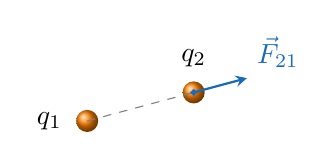
\begin{tikzpicture}[scale=0.7,>=stealth]
      \def\l{2}
      \def\ang{15}
      \shade[ball color=orange] (0,0) circle (.2) node[left=2mm] {$q_1$};
      \shade[ball color=orange] (\ang:\l) circle (.2) node[above=2mm] {$q_2$};
      \draw[dashed,gray] (0,0) -- (\ang:\l);
      \draw[thick,cyan!45!blue] (\ang:\l) circle (1pt);
      \draw[thick,cyan!45!blue,->] (\ang:\l) -- (\ang:\l+1) node[above right] {$\vec{F}_{21}$}; 
    \end{tikzpicture}
    \caption{La fuerza eléctrica}
    \label{fig_ej_cargas_vectoriales}
  \end{marginfigure}
\end{example}
Esto es importante tenerlo en cuenta ya que si se quiere saber la fuerza total sobre una carga \( q \) debido a varias cargas, se debe sumar vectorialmente las fuerzas individuales. La fuerza total sobre una carga \( q \) debido a un conjunto de cargas \( Q_i \) es:

\begin{equation}
  \vec{F} = \sum_i k \frac{|q \cdot Q_i|}{r_i^2} \hat{\mathbf{r_i}}
\end{equation}

\begin{figure}[ht]
  \centering
    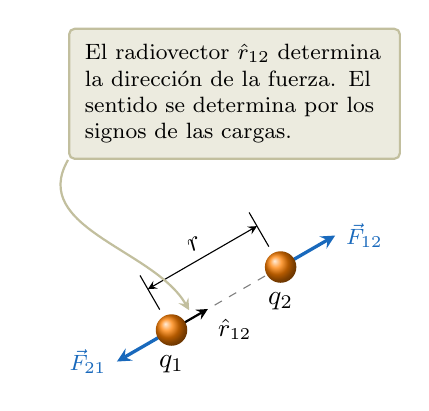
\begin{tikzpicture}[>=stealth]
    \def\h{.8}
    \def\l{1.6}
    \coordinate (r) at (30:\l/5);
    \draw[dashed,gray] (0,0) -- (30:\l);
    \draw[thin] (0,0) ++(120:.3) -- (120:\h); 
    \draw[thin] (30:\l) ++(120:.3) -- +(120:\h-.3);
    \draw[thin,<->] (120:.6) -- node[above,sloped] {$r$} +(30:\l);
    \draw[thick,->] (0,0) -- (30:\l/3) node[below right,font=\small] {$\hat{r}_{12}$};
    \draw[cyan!45!blue,->,very thick] (0,0) -- (210:\l/2) node[left,font=\footnotesize] {$\vec{F}_{21}$};
    \draw[cyan!45!blue,->,very thick] (30:\l) -- +(30:\l/2) node[right,font=\footnotesize] {$\vec{F}_{12}$};
    \shade[ball color=orange] (0,0) circle (.2) node[below=2mm] {$q_1$};
    \shade[ball color=orange] (30:\l) circle (.2) node[below=2mm] {$q_2$};
    
    \node (cartel) [
      font=\footnotesize,
      text width=3.8cm,
      align=left,
      fill=yellow!40!black!14,
      draw=yellow!40!black!46,
      thick,
      rounded corners=2pt,
      inner sep=2mm
      ]
      at (.8,3) {
        El radiovector $\hat{r}_{12}$ determina la dirección de la fuerza. El sentido se determina por los signos de las cargas.
    };

    \draw[->, thick, color=yellow!40!black!46, shorten >=3pt] 
             (cartel.south west) to[out=240, in=120] (r);
  \end{tikzpicture}
  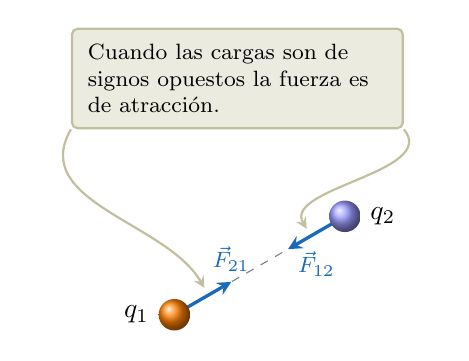
\begin{tikzpicture}[>=stealth]
    \def\h{.8}
    \def\l{2.5}
    \coordinate (r) at (30:\l/5);
    \draw[dashed,gray] (0,0) -- (30:\l);
    \draw[cyan!45!blue,->,very thick] (0,0) -- (30:\l/3) node[above,font=\footnotesize] {$\vec{F}_{21}$};
    \draw[cyan!45!blue,->,very thick] (30:\l) -- node[below=1mm,font=\footnotesize] {$\vec{F}_{12}$} +(210:\l/3);
    \shade[ball color=orange] (0,0) circle (.2) node[left=2mm] {$q_1$};
    \shade[ball color=blue!40] (30:\l) circle (.2) node[right=2mm] {$q_2$};
    
    \node (cartel) [
      font=\footnotesize,
      text width=3.8cm,
      align=left,
      fill=yellow!40!black!14,
      draw=yellow!40!black!46,
      thick,
      rounded corners=2pt,
      inner sep=2mm
      ]
      at (.8,3) {Cuando las cargas son de signos opuestos la fuerza es de atracción.};

    \draw[->, thick, color=yellow!40!black!46, shorten >=3pt] 
             (cartel.south west) to[out=240, in=120] (r);
    \draw[->, thick, color=yellow!40!black!46, shorten >=3pt] 
             (cartel.south east) to[out=310, in=120] (30:4*\l/5);
  \end{tikzpicture}

  \caption{Determinación de la dirección y sentido de la fuerza eléctrica entre dos cargas puntuales.}
  \label{fig:coulomb}
\end{figure}

Note que en la figura \ref{fig:coulomb} el subíndice de la fuerza no se lee de la misma forma que en el ejemplo \ref{ej_ley_de_coulomb}. En el caso de la figura se lee 
\begin{quote}
  ``\(F_{21}\) es la fuerza que ocasiona la carga \(q_2\) sobre la carga \(q_1\)''
\end{quote}
Esto no tiene diferencias significativas sobre la notación del ejemplo, y usted puede usar la notación que le resulte más cómoda.

\subsection{Carga eléctrica}

La carga eléctrica es una propiedad fundamental de la materia que determina la interacción electromagnética entre partículas. Se trata de una magnitud escalar que puede ser de dos tipos: positiva o negativa. Las partículas con carga del mismo signo se repelen, mientras que las de signo opuesto se atraen.

La unidad de carga eléctrica en el Sistema Internacional (SI) es el coulomb (\unit{\coulomb}). La carga elemental está representada por la carga del electrón (\( -e = -\qty{1.602e-19}{\coulomb} \)) y la del protón (\( e = +\qty{1.602e-19}{\coulomb} \)).

\begin{center}
  \setlength{\arrayrulewidth}{1pt}
  \renewcommand{\arraystretch}{1.3}
  \arrayrulecolor{gray}

  \begin{tabular}{ c c c }
    \hline
    \rowcolor{asparagus!30}
    Partícula  & Carga (\unit{\coulomb})           & Masa (\unit{\kilogram})   \\ \hline
    Electrón (e)        & \(-e = -1.602 \times 10^{-19}\)   & \(9.109 \times 10^{-31}\) \\
    Protón (p)          & \(+e = +1.602 \times 10^{-19}\)   & \(1.672 \times 10^{-27}\) \\
    Neutrón (n)         & \(0\)                             & \(1.675 \times 10^{-27}\) \\ \hline
  \end{tabular}
\end{center}
